\documentclass{report}
\usepackage{natbib}
\title{DisperseR: Calculating Seed Dispersal In R}
\author{Samantha L. Davis}
\usepackage{Sweave}
\begin{document}
\maketitle
\tableofcontents
\Sconcordance{concordance:disperseRmanual.tex:disperseRmanual.Rnw:%
1 4 1 1 0 35 1 1 2 1 0 2 1 11 0 1 1 12 0 1 2 4 1 1 3 11 0 1 2 4 0 1 2 5 %
1 1 6 5 0 1 1 12 0 1 2 6 1 1 5 4 0 1 6 4 0 1 1 11 0 1 1 12 0 1 2 5 1 1 %
4 3 0 1 1 11 0 1 1 9 0 1 4 2 0 1 1 11 0 1 1 10 0 1 2 6 1 1 2 1 0 2 2 10 %
0 1 1 5 0 1 2 11 0 1 1 6 0 1 2 10 1 1 2 19 0 1 1 16 0 1 3 1 0 1 1 1 3 1 %
0 1 3 2 0 1 4 1 0 1 3 2 0 1 3 4 0 1 2 2 1 1 2 1 0 1 1 5 0 1 1 16 0 1 4 %
2 0 1 2 1 0 1 3 5 0 1 2 3 1 1 2 5 0 1 2 3 1 1 6 5 0 1 3 2 0 1 1 6 0 1 2 %
1 1 1 2 4 0 1 2 6 1}


\chapter{Introduction}

This is a small package intended to help users calculating seed dispersal in R. Although the R base machinery is capable of doing so, this package streamlines the process and enables you to focus more on the important aspects of data analysis instead of data generation or clean-up.

This code operates as follows. Ideally, you'll need a dataframe that contains the following data: (x,y) coordinates of each tree and seedling in a plot; and dbh measurements of any tree large enough. A tree is any individual that can be measured for diameter at breast height, and all trees are assumed to be reproductively active; a seedling is any individual that is new in the calendar year.

Spatial seed dispersal is characterized by a single equation,

\begin{equation}
\label{eq:dispersal}
R_i = STR * \sum\limits_{k=1}^T\left( \frac{DBH_k}{30}\right) ^\beta e^{-Dm_{ik}^3} * \left( \frac{1}{n}\right)
\end{equation}

where \textit{n} is a normalizer function that standardizes the equation to values between 0 and 1,

\begin{equation}
n = \int\limits_{0}^\infty e^{-Dm_{ik}^3} \nonumber
\end{equation}

and where \textit{STR} is the standardized number of tree recruits, \textit{DBH} is the diameter at breast height, \textit{$\beta$} is a modifier of DBH and STR,  \textit{D} is a species-specific parameter estimated by this equation, and \textit{m} is the distance between the measured point \textit{i} and adult tree \textit{k}, summed over each adult tree (\textit{k}=1 to \textit{T} adult trees). These equations were originally established by \citet{Ribbens1994}, in an experiment where seedling per $m^2$ along a belt transect were correlated to the number and size of any adults within a $20 m$ radius.

The first piece of the equation, containing STR, establishes the number of recruits produced for a tree of a standard DBH (30cm), and the second piece of the equation establishes the mean density of recruits found in a $1 m^2$ quadrat centered at \textit{m} distance away from the parent tree. Finally, $\frac{1}{n}$ serves as a normalizer to standardize the equation across species.

The parameters \textit{STR} and {D} are both needed by SORTIE-ND, an individual tree neighborhood dynamics forest gap model (say that five times fast!), to calculate seed dispersal for target species in its simulations. SORTIE-ND, unfortunately, does not come packaged with a magic bullet that offers species-specific parameters, and therefore, we must parameterize the model ourselves. This package is intended to help create estimates of both \textit{STR} and \textit{D} quickly, so that other parameters may be addressed.

What follows is a list of functions alongside example usage. To start, you must import or generate a plot map of all trees in a given area. This plot map must include a species identifier, an x coordinate, a y coordinate, and DBH (or NA) for each individual.

\chapter{Using Coherent Plot Map Data}

\section{Generating Plot Map}

\subsection{generatePlotMap}
We can generate a sample plot easily with generatePlotMap(). As you can see below, this function generates a plot map with NA's for seedlings and actual values of DBH for adult trees. See ?generatePlotMap() for information on how to customize your random plot map.
\begin{Schunk}
\begin{Sinput}
> library(disperseR)
> myplot <- generatePlotMap()
> head(myplot)
\end{Sinput}
\begin{Soutput}
  treeid species         x         y dbh    stage
1      1       1   4.13521 661.91449  NA seedling
2      2       1 768.01953 978.57594  NA seedling
3      3       1 423.94914 418.09895  NA seedling
4      4       1 980.03977 534.79190  NA seedling
5      5       1 511.07972  13.71672  NA seedling
6      6       1 632.19266  57.73108  NA seedling
\end{Soutput}
\begin{Sinput}
> tail(myplot)
\end{Sinput}
\begin{Soutput}
    treeid species        x         y      dbh stage
745    745       5 475.7327 109.70244 56.50662  tree
746    746       5 414.8146 394.20455 62.82194  tree
747    747       5 778.1309 290.82872 12.81504  tree
748    748       5 218.7070 935.61995 50.04510  tree
749    749       5 230.3108  85.71495 99.50670  tree
750    750       5 651.8597 827.16404 91.08299  tree
\end{Soutput}
\end{Schunk}

If you do have your own data, just make sure that it matches the column names of the plot map generated above, and also the data types. You can check the structure of a dataframe using str() and then as.numeric() or as.character() to adjust as needed. In our case, you need five columns: treeid, species, x, y, and dbh. x, y, and dbh should all be numeric. ``species'' can be a character vector or a numeric vector, as long as the species names are unique. ``treeid'' is a unique identifier for each tree. If you generate randomly, it will match the rownumbers of your resulting data.frame. You'll also need a ``stage'' column, which is just a shortcut for figuring out if a record is for a seedling or a tree.

\begin{Schunk}
\begin{Sinput}
> ## exploring the structure of myplot
> str(myplot)
\end{Sinput}
\begin{Soutput}
'data.frame':	750 obs. of  6 variables:
 $ treeid : int  1 2 3 4 5 6 7 8 9 10 ...
 $ species: int  1 1 1 1 1 1 1 1 1 1 ...
 $ x      : num  4.14 768.02 423.95 980.04 511.08 ...
 $ y      : num  661.9 978.6 418.1 534.8 13.7 ...
 $ dbh    : num  NA NA NA NA NA NA NA NA NA NA ...
 $ stage  : chr  "seedling" "seedling" "seedling" "seedling" ...
\end{Soutput}
\begin{Sinput}
> ## if we needed to convert a column
> myplot$species <- as.numeric(myplot$species)
\end{Sinput}
\end{Schunk}

\section{Sampling The Plot Map}

Now that we have a plot map ready, we need to be able to sample the plot.  \citet{Ribbens1994} sampled using a belt transect, stopping every so often to count all of the seedlings in a $1 m^2$ plot, and all adult trees within $20m$ of the seedling plot. We have an advantage, in that we have the exhaustive map and can just sample for every individual or clump of seedlings there is.

We can do this with a ``find and eliminate'' approach. For each possible seedling, subsetted from the plot map, we can search around it at ``m'' distance to see if there are other seedlings. We can count the total number of seedlings in that box, store the (x,y) and number (n) in a data.frame, prevent the counted seedlings from getting re-counted, and move to the next row. This functionality is wrapped up in the findSeedPlots() function in disperseR, demonstrated below. Remember, your input data.frame will need all of the columns generated by generatePlotMap().

\begin{Schunk}
\begin{Sinput}
> ## make a sample seed data.frame by subsetting the included
> ## expandedTrees data.frame..
> seeds <- myplot[myplot$stage=="seedling",]
> ## we'll need this one later...
> adults <- myplot[myplot$stage=="tree",]
> ## show the start of results
> myseedplots <- findSeedPlots(seeds, 1)
> head(myseedplots)
\end{Sinput}
\begin{Soutput}
          x         y n
1   4.13521 661.91449 1
2 768.01953 978.57594 1
3 423.94914 418.09895 1
4 980.03977 534.79190 1
5 511.07972  13.71672 1
6 632.19266  57.73108 1
\end{Soutput}
\begin{Sinput}
> ## What are the possible densities of our seedplots?
> unique(myseedplots$n)
\end{Sinput}
\begin{Soutput}
[1] 1
\end{Soutput}
\end{Schunk}



Now that we have seedling density in our subplots, we need to figure out how many possible parent trees there are for each of the positive hits. We can do that using the findAdultTrees() function.

\subsection{findAdultTrees}

The findAdultTrees() function works by searching a full plot for trees that are ``m'' distance away from the points provided (seedling plot points).

\begin{Schunk}
\begin{Sinput}
> parentTrees <- findAdultTrees(myseedplots, adults, 20)
> head(parentTrees)
\end{Sinput}
\begin{Soutput}
  treeid ri         m      dbh
1     79  1 16.159211 34.72850
2    410  1 10.715594 35.91574
3    392  1 16.045922 72.33590
4    407  1 18.748185 18.88682
5    113  1 18.330470 54.66067
6    531  1  7.969868 85.19551
\end{Soutput}
\begin{Sinput}
> nrow(parentTrees)
\end{Sinput}
\begin{Soutput}
[1] 66
\end{Soutput}
\end{Schunk}

Now, you can see that the random plot map that we've generated doesn't work too well on its default values at getting ``good'' values for this equation. ``ri'', in particular, should have more than one unique value if it's going to be used as a predictor value. Now that we've shown proof of concept for these functions, however, we're going to get around the limitation of random data by using some data that comes in the package, known as expandedTrees. This data is obfuscated real data, as you'll see below.

\section{Calculating Parameters for the Ribbens Equation}

Unfortunately, because the data above are randomly generated, they will not allow a NLS model to converge on a meaningful parameter set. To get around this and demonstrate the model, we've included a large plot-year dataset called ``expandedTrees''.  This dataset represents unique data when subsetted at the ``plot'' and ``measyear'' columns. You can use ?expandedTrees to find out more about the dataset and how it functions. expandedTrees is generated from ssdAllTrees and ssdPlotDesc, so check those data.frames out too if you need more information.

Since expandedTrees is organized by plot and year, we can take one of those plot-year combinations and run the model. We will also need to generate a seedling map and all of the other steps from above.

Let's look at expandedTrees, and take the first plot-year combination available.

\begin{Schunk}
\begin{Sinput}
> head(expandedTrees)
\end{Sinput}
\begin{Soutput}
      plot subplot treeid species ingrowth firstrec deathyear        x        y
2 crackers       1      1    ABCO       NA     1992        NA 89902.54 48132.50
3 crackers       1      1    ABCO       NA     1992        NA 89902.54 48132.50
4 crackers       1      1    ABCO       NA     1992        NA 89902.54 48132.50
5 crackers       1      1    ABCO       NA     1992        NA 89902.54 48132.50
6 crackers       1      1    ABCO       NA     1992        NA 89902.54 48132.50
7 crackers       1      2    ABCO       NA     1992        NA 89908.76 48133.72
  measyear dbh stage
2     1992 4.4  tree
3     1997 5.0  tree
4     2002 5.6  tree
5     2007 6.0  tree
6     2012 6.2  tree
7     1992 8.7  tree
\end{Soutput}
\begin{Sinput}
> str(expandedTrees)
\end{Sinput}
\begin{Soutput}
'data.frame':	51493 obs. of  12 variables:
 $ plot     : chr  "crackers" "crackers" "crackers" "crackers" ...
 $ subplot  : num  1 1 1 1 1 1 1 1 1 1 ...
 $ treeid   : num  1 1 1 1 1 2 2 2 2 2 ...
 $ species  : chr  "ABCO" "ABCO" "ABCO" "ABCO" ...
 $ ingrowth : num  NA NA NA NA NA NA NA NA NA NA ...
 $ firstrec : num  1992 1992 1992 1992 1992 ...
 $ deathyear: num  NA NA NA NA NA NA NA NA NA NA ...
 $ x        : num  89903 89903 89903 89903 89903 ...
 $ y        : num  48132 48132 48132 48132 48132 ...
 $ measyear : num  1992 1997 2002 2007 2012 ...
 $ dbh      : num  4.4 5 5.6 6 6.2 8.7 9.1 9.8 10.4 11.1 ...
 $ stage    : chr  "tree" "tree" "tree" "tree" ...
\end{Soutput}
\begin{Sinput}
> ## get unique plot/year combos
> plotlist <- unique(expandedTrees[,c("plot", "measyear")])
> rownames(plotlist) <- 1:nrow(plotlist)
> ## count the number of adult trees in a plot/year combination
> plotlist$tree <- NA
> for(i in 1:nrow(plotlist)){
+   plotlist[i, "tree"] <- nrow(
+                           expandedTrees[
+                            expandedTrees$plot==plotlist[i, "plot"] &
+                            expandedTrees$measyear==plotlist[i, "measyear"] &
+                            expandedTrees$stage=="tree",])
+ }
> ## get number of seedlings in a plot/year combo
> plotlist$seedlings <- NA
> for(i in 1:nrow(plotlist)){
+   plotlist[i, "seedlings"] <- nrow(
+                                expandedTrees[
+                                expandedTrees$plot==plotlist[i, "plot"] &
+                                expandedTrees$measyear==plotlist[i, "measyear"] &
+                                expandedTrees$stage=="seedling",])
+ }
> ## eliminate any plots that have only trees or seedlings
> plotlist <- plotlist[plotlist$tree!=0 & plotlist$seedlings!=0,]
\end{Sinput}
\end{Schunk}

For now, let's take a large plot, like trinity, in one of its middle years. The data.frame knows exactly when seedlings established in middle years, because plots were checked years for establishment. Let's do trinity in 2001:

\begin{Schunk}
\begin{Sinput}
> trinity01 <- expandedTrees[
+               expandedTrees$plot=="trinity" &
+               expandedTrees$measyear==2001,]
> nrow(trinity01[trinity01$stage=="seedling",])
\end{Sinput}
\begin{Soutput}
[1] 431
\end{Soutput}
\begin{Sinput}
> str(trinity01)
\end{Sinput}
\begin{Soutput}
'data.frame':	2402 obs. of  12 variables:
 $ plot     : chr  "trinity" "trinity" "trinity" "trinity" ...
 $ subplot  : num  1 1 1 1 1 1 1 1 1 1 ...
 $ treeid   : num  1532 1534 1535 1536 1537 ...
 $ species  : chr  "ABCO" "ABCO" "ABCO" "ABCO" ...
 $ ingrowth : num  NA NA NA NA NA NA NA NA NA NA ...
 $ firstrec : num  1991 1991 1991 1991 1991 ...
 $ deathyear: num  NA NA 2012 NA 2003 ...
 $ x        : num  88904 88903 88900 88900 88902 ...
 $ y        : num  48744 48741 48738 48737 48736 ...
 $ measyear : num  2001 2001 2001 2001 2001 ...
 $ dbh      : num  15.3 13.9 7.5 15.5 2 18.3 32.5 10.6 22.5 17.2 ...
 $ stage    : chr  "tree" "tree" "tree" "tree" ...
\end{Soutput}
\begin{Sinput}
> ## set up for plot
> ## by stage
> trinity01$colors <- ifelse(trinity01$stage=="seedling", "red", "blue")
> ## by species
> specieslist <- unique(trinity01$species)
> for(i in 1:length(specieslist)){
+   trinity01[trinity01$species==specieslist[i],"pch"] <- as.numeric(i)
+ }
\end{Sinput}
\end{Schunk}


Now, let's take a look at the distribution of seedlings and adults by species. This is just a simple graph of trinity01, not scaled to dbh at all. See the code above for the color/species designations

\begin{Schunk}
\begin{Sinput}
> plot(trinity01$x, trinity01$y, pch=trinity01$pch, col=trinity01$colors)
\end{Sinput}
\end{Schunk}
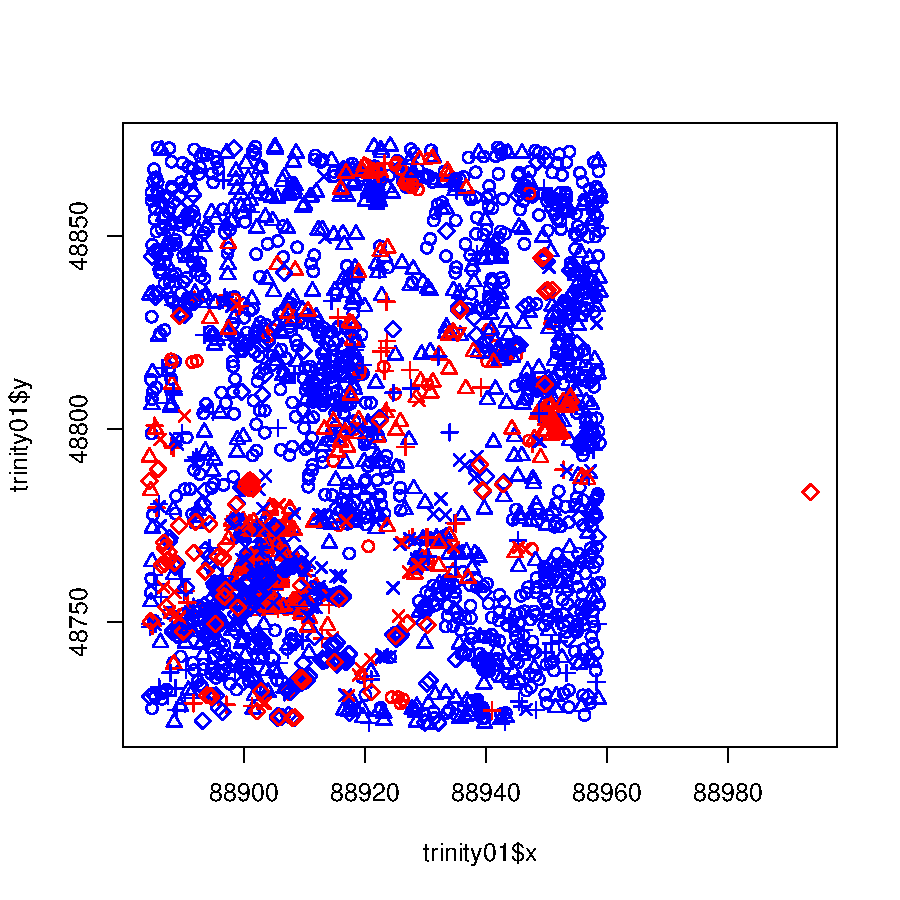
\includegraphics{disperseRmanual-007}


And now let's separate out the seedlings from trees, and run our scripts to get parentTrees. The scripts also only deal with a single species, so we'll pick one.

\begin{Schunk}
\begin{Sinput}
> ## get seeds and adults ready
> trinSeeds <- trinity01[trinity01$stage=="seedling" &
+                          trinity01$species=="ABCO", ]
> trinAdults <- trinity01[trinity01$stage=="tree" &
+                          trinity01$species=="ABCO", ]
> seedlingPlots <- findSeedPlots(trinSeeds, 1)
> parentTrees <- findAdultTrees(seedlingPlots, trinAdults, 20)
> ## check that there are multiple seedling densities,
> ## and parentTrees looks right.
> str(parentTrees)
\end{Sinput}
\begin{Soutput}
'data.frame':	3352 obs. of  4 variables:
 $ treeid: chr  "1532" "1534" "1535" "1536" ...
 $ ri    : num  1 1 1 1 1 1 1 1 1 1 ...
 $ m     : num  15 15.8 14.5 15.9 18 ...
 $ dbh   : num  15.3 13.9 7.5 15.5 2 18.3 32.5 10.6 22.5 3 ...
\end{Soutput}
\begin{Sinput}
> unique(parentTrees$ri)
\end{Sinput}
\begin{Soutput}
[1] 1 2 4
\end{Soutput}
\end{Schunk}

Yay, we have a functioning parentTrees dataframe that we can use to estimate parameters! Onto the parameters. If you remember from above, we are trying to to find parameters for this equation:

\begin{equation}
\label{eq:dispersal-repeat}
R_i = STR * \sum\limits_{k=1}^T\left( \frac{DBH_k}{30}\right) ^\beta e^{-Dm_{ik}^3} * \left( \frac{1}{n}\right)
\end{equation}

To estimate STR, $\beta$, and D, we'll need to run a non-linear least squares model. But, to be honest, those are super-breakable and suck in R. If you notice, however, this equation only non-linear because of the second half ($e^{...}$). As all ecologists love to do, we can take the natural log of boths sides of this equation and turn it into a linear model that looks something like this:

\begin{equation}
\label{eq:log-disp}
ln(R_i) = ln(STR) + \beta * ln(\frac{DBH}{30}) + D * m^3
\end{equation}

This transformation means that the parameters we are estimating, $\beta$, STR, and D, are all related linearly to the other parameters. In layman's terms, that means that we can now predict the parameters using the much more robust and unbreakable function glm() in R. The formula we'll be using looks like this:

\begin{Schunk}
\begin{Sinput}
> formula <- "log(ri)~log(dbh/30) + m^3"
\end{Sinput}
\end{Schunk}

As a reminder, the log() function in R gives the natural log (ln, or $log_e$), not the $log_{10}$ value.

We will do the normalizer afterwards, because it should not affect the outcome of the model. Now that we have the data.frame and the model, it's a simple matter of running it, then taking a look at the transformed parameters and converting them back to the form we need them in.

\begin{Schunk}
\begin{Sinput}
> myModel <- glm(formula, data=parentTrees)
> summary(myModel)
\end{Sinput}
\begin{Soutput}
Call:
glm(formula = formula, data = parentTrees)

Deviance Residuals: 
    Min       1Q   Median       3Q      Max  
-0.2281  -0.1608  -0.1381  -0.1120   1.2928  

Coefficients:
             Estimate Std. Error t value Pr(>|t|)    
(Intercept)  0.175139   0.018673   9.379  < 2e-16 ***
log(dbh/30) -0.013730   0.005548  -2.475 0.013385 *  
m           -0.003941   0.001120  -3.519 0.000438 ***
---
Signif. codes:  0 ‘***’ 0.001 ‘**’ 0.01 ‘*’ 0.05 ‘.’ 0.1 ‘ ’ 1

(Dispersion parameter for gaussian family taken to be 0.1053276)

    Null deviance: 353.31  on 3333  degrees of freedom
Residual deviance: 350.85  on 3331  degrees of freedom
  (18 observations deleted due to missingness)
AIC: 1962.7

Number of Fisher Scoring iterations: 2
\end{Soutput}
\end{Schunk}

As you can see, that's about as simple as you can get! But what do these parameters mean? The intercept in this is actually the ln(STR), so we need to do $e^i$ to find the value of STR. The parameter generated for dbh is representative of $\beta$ without transformation. And the parameter generated for m is equivalent to -D, so we need to get the negative value for it to be equal to D.

\begin{Schunk}
\begin{Sinput}
> STR <- exp(myModel$coefficients[1])
> beta <- myModel$coefficients[2]
> D <- -myModel$coefficients[3]
> STR
\end{Sinput}
\begin{Soutput}
(Intercept) 
   1.191412 
\end{Soutput}
\begin{Sinput}
> beta
\end{Sinput}
\begin{Soutput}
log(dbh/30) 
-0.01372956 
\end{Soutput}
\begin{Sinput}
> D
\end{Sinput}
\begin{Soutput}
          m 
0.003941383 
\end{Soutput}
\begin{Sinput}
> 
\end{Sinput}
\end{Schunk}

\chapter{Using Seed Trap Data}

In some cases, your seed data will be completely separate from your individual tree map. Unlike Eastern forests, mountain pine forests often grow very slowly, and it can take a long time for seedlings to emerge and begin growth. As a result, you may commonly miss seedlings if you're mapping, or it may be difficult to tell when they emerged. In these cases, you can use seed traps to estimate seedling dispersal. One major caveat is that the number of viable seeds caught may correlate with, but will not match the true seedling establishment rate.

Now, to use seed trap data, you must know where each seed trap is located in your plots. In the data that we are using, we know the plot layout for each individual plot and their respective subplots, we know which subplots have seed traps, and we know the placement of seedtraps within subplots. However, we do not know the precise (x,y) locations of seed traps. We also have a complicating factor: in some cases, because these are real data, the coordinates are in UTMN/UTME, but not all of our plots are aligned perfectly on a N-S, E-W orientation.

Now, all other things aside, the easiest way to approach this problem is to rotate our plots to make them align correctly. This is the easiest way because a function to locate the seed traps, given the subplot locations, has already been established.

We can approach this problem using the rotatePlot() function. If we look through our plots, we see that the first plot in expandedTrees, "bellow" is rotated. We will fix it using rotatePlot().

\begin{Schunk}
\begin{Sinput}
> bellow <- expandedTrees[expandedTrees$plot=="bellow",]
> ## make a color column, set it to "black"
>   bellow$col <- "black"
> ## Set the leftmost points, the points we're rotating on, to red
>   bellow[bellow$x==min(bellow$x), "col"] <- "red"
> ## Rotate plot
> ## We need the "true southwestern corner", which can be found in ssdPlotDesc
>   rotatebellow <- rotatePlot(bellow,
+                              truesw=c(
+                                ssdPlotDesc[ssdPlotDesc$plot=="bellow", "x"],
+                                ssdPlotDesc[ssdPlotDesc$plot=="bellow", "y"]
+                                ))
\end{Sinput}
\end{Schunk}

\newpage
\begin{Schunk}
\begin{Sinput}
> ## plot
> par(mfrow=c(2,1))
> plot(bellow$x, bellow$y, col=bellow$col)
> plot(rotatebellow$x, rotatebellow$y, col=rotatebellow$col)
> par(mfrow=c(1,1))
\end{Sinput}
\end{Schunk}
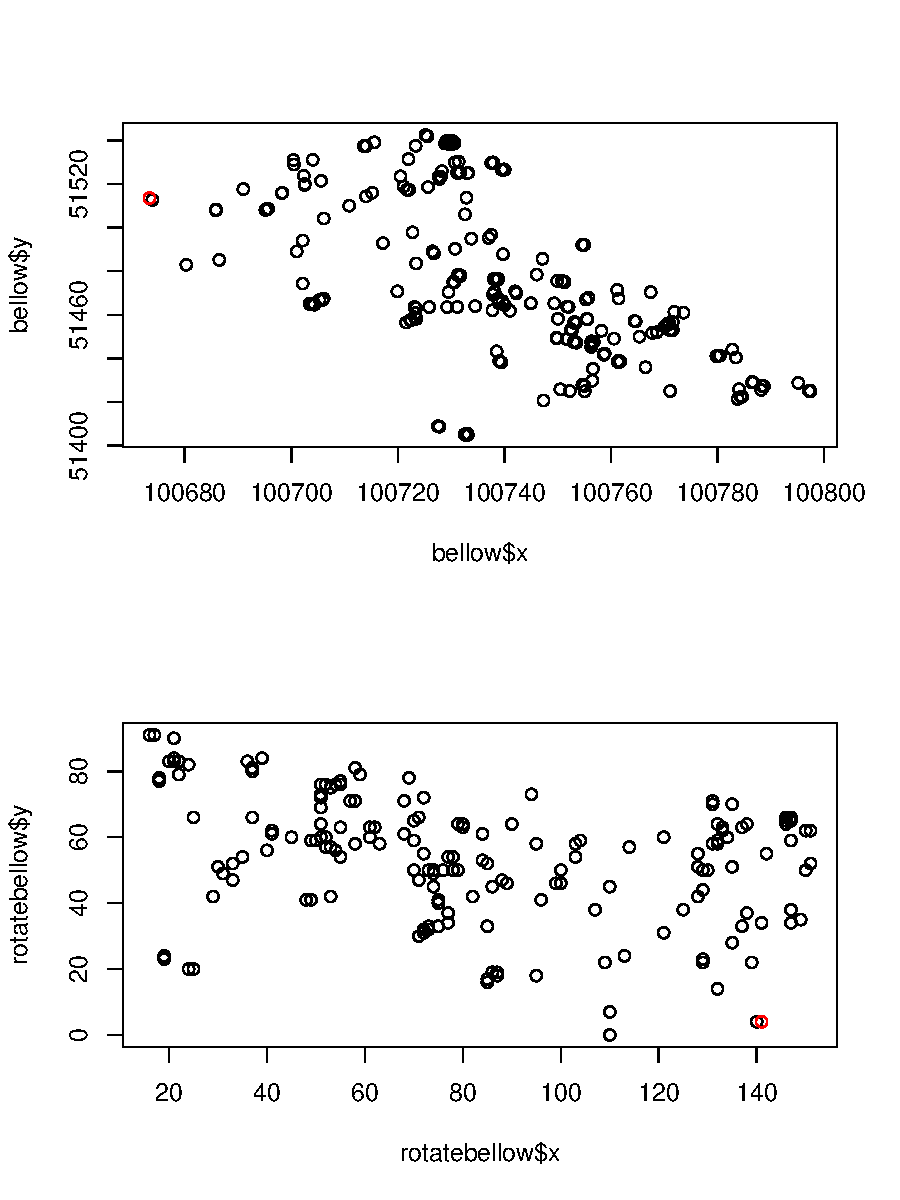
\includegraphics{disperseRmanual-013}

Ok, so we can successfully rotate the plots. The other important thing to note is that the only things altered between bellow and rotatebellow are their (x,y) coordinates. Everything else, all of the extraneous columns, like "col", are kept the same. That means, in data.frames where we have subplot information, we can figure out where the subplots are in both rotated and unrotated space. Luckily, expandedTrees does have subplot information! So, let's get a feel for the subplot layout in bellow.

\begin{Schunk}
\begin{Sinput}
> rainbowColors <- rainbow(max(bellow$subplot))
> palette(rainbowColors)
> plot(rotatebellow$x, rotatebellow$y, col=rotatebellow$subplot)
> 
\end{Sinput}
\end{Schunk}
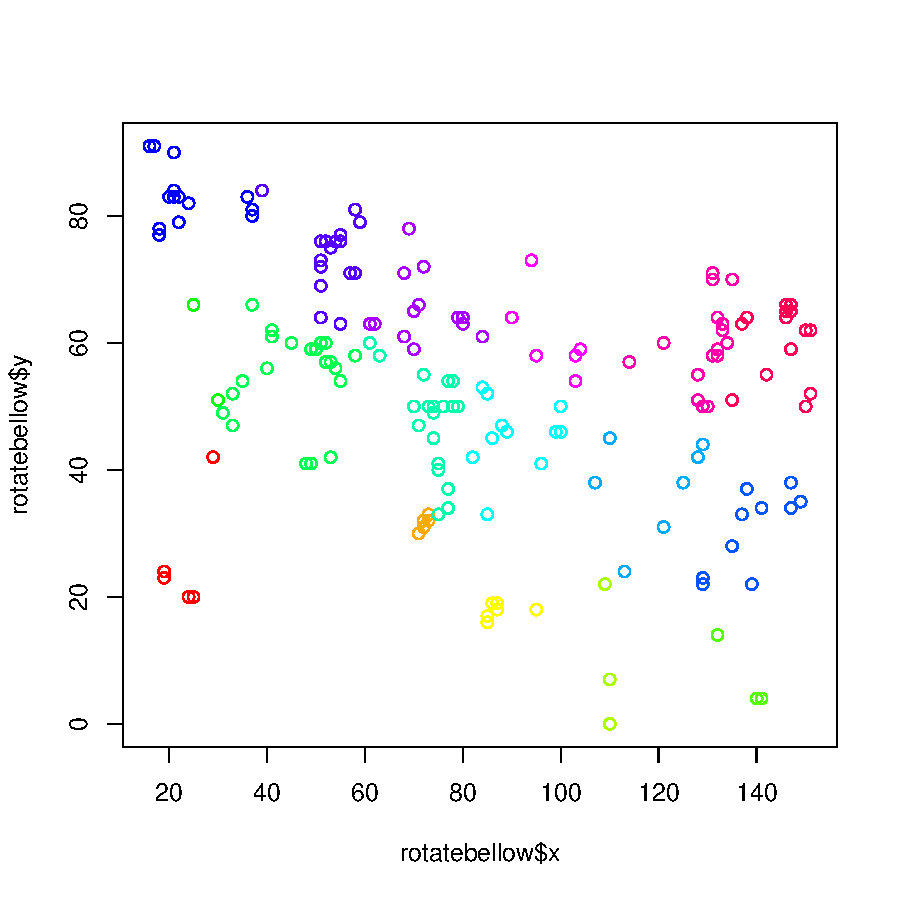
\includegraphics{disperseRmanual-014}

We can see from the figure that rotate bellow's subplot 1 starts in the top left, fills through the bottom, and does three columns like that. bellow is approximately 75 meters along the x axis and 150 meters along the y axis. Since we know each subplot is 25x25m, we can generate a subplot corners dataframe that knows the corners of each of the subplot boundaries. This is the data.frame we'll need to find the trap locations.

Let's check and see what the dimensions on these plots are, and if they are truly made of 25x25 subplots.

\begin{Schunk}
\begin{Sinput}
> ##get names of subplots
> plotnames <- unique(expandedTrees$plot)
> ##quick function to calculate ranges of x's and y's
> getRange <- function(x){
+   store <- max(x) - min(x)
+   return(store)
+ }
> ## set up response table
> plotdimensions <- data.frame(
+   plot=plotnames,
+   xrange=0,
+   yrange=0,
+   stringsAsFactors=FALSE)
> ##do loop through
> for(i in 1:length(plotnames)){
+   plotdimensions[i, "xrange"] <- getRange(
+     expandedTrees[expandedTrees$plot==plotnames[i],"x"])
+     plotdimensions[i, "yrange"] <- getRange(
+       expandedTrees[expandedTrees$plot==plotnames[i],"y"])
+ }
> ## view plot dimensions
> plotdimensions
\end{Sinput}
\begin{Soutput}
        plot   xrange  yrange
1   crackers 133.3200 133.790
2    trinity 109.7311 149.999
3    realtor  99.5330  99.610
4     bellow 124.0920 137.500
5     palate  80.9180 102.610
6  reclusive 110.3090 121.350
7     octane 193.0020 111.920
8     sodium  99.2630  99.270
9   distress  99.6390  99.520
10     gravy  99.7690  99.740
11   trigger  89.6610 128.040
12     rigid  84.3110 223.790
\end{Soutput}
\begin{Sinput}
> 
> 
\end{Sinput}
\end{Schunk}

So it seems like some are, and some are not. So we better build a program to draw subplots that can handle the weird ones. We built a few functions to handle drawing boxes. These functions are demonstrated below.

\begin{Schunk}
\begin{Sinput}
> ## get the min and max values for each corner.
> corners <- c(0, max(rotatebellow$x), 0, max(rotatebellow$y))
> ## get the box corners based on a 25 m incremented subplot:
> ## ## get coords
>   xcoords <- getSubplotCoords(corners[1:2], increment=25)
>   ycoords <- getSubplotCoords(corners[3:4], increment=25)
>   xcoords
\end{Sinput}
\begin{Soutput}
[1]   0  25  50  75 100 125 150 175
\end{Soutput}
\begin{Sinput}
>   ycoords
\end{Sinput}
\begin{Soutput}
[1]   0  25  50  75 100
\end{Soutput}
\begin{Sinput}
> ##build the boxes and check our work.
> 
>   bellowSubplots <- buildBoxes(xcoords, ycoords)
>   ## check our work
> plot(rotatebellow$x, rotatebellow$y, pch=".", xlim=c(corners[1], corners[2]), ylim=c(corners[3], corners[4]))
> points(bellowSubplots$POINT_X, bellowSubplots$POINT_Y, col="red", pch=4)
> 
\end{Sinput}
\end{Schunk}
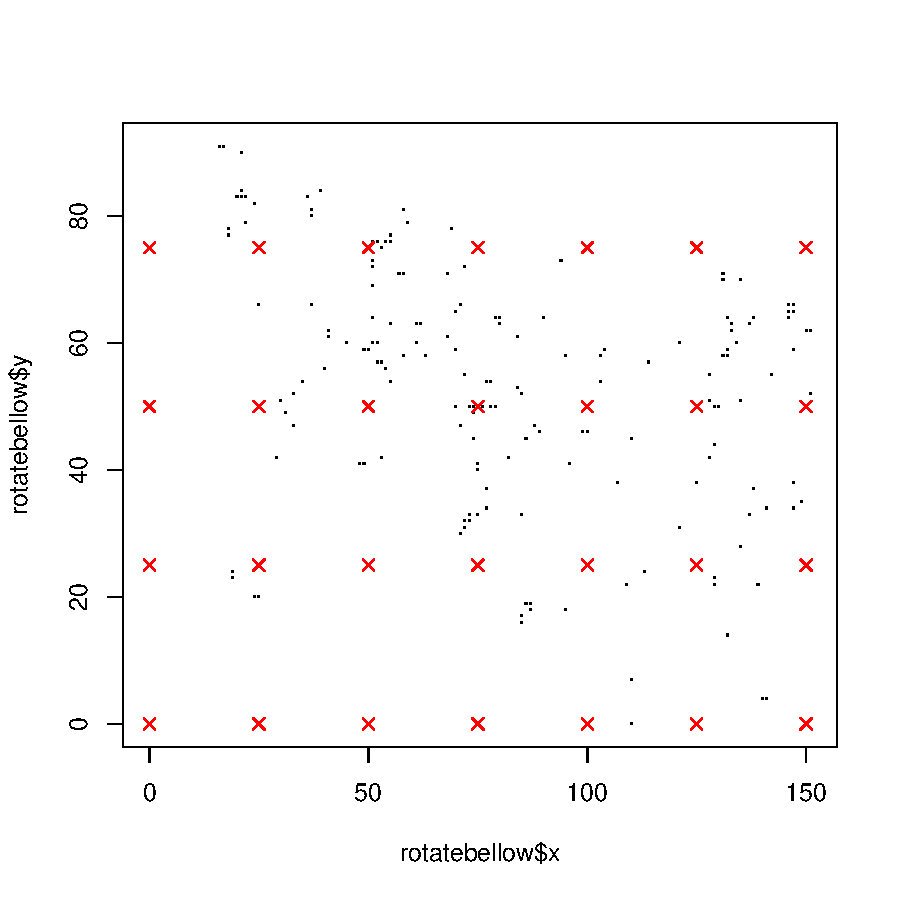
\includegraphics{disperseRmanual-016}


\bibliographystyle{sty/ecology}
\bibliography{disperseRmanual}
\end{document}
